\hyperdef{directed}{graph}{\chapter{Relations and Directed Graphs}}

\section{Digraphs} 

Informally, a \term{directed graph}, called a \emph{digraph} for short, is
a bunch of dots with arrows going from one dot to another, as in
Figure~\ref{picdigraphg}, for example.

\begin{figure}[htbp]
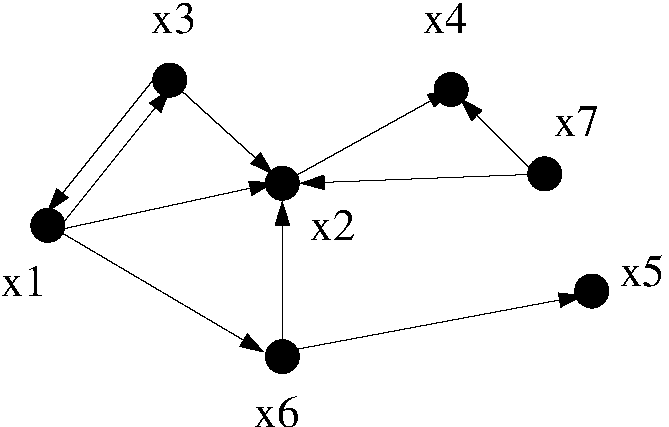
\includegraphics[height=1,5in]{webGraph.pdf}
\caption{Picture of a digraph, $D$.}
\label{picdigraphg}
\end{figure}

%\mfigure{!}{1.5in}{figures/digraph-ps2f03.pdf}

%\mfigure{!}{1.5in}{figures/webGraph.pdf}

For Mathematical purposes, we don't really care how the points and arrows
are laid out ---only which arrows point to which points.  For the digraph,
$D$, of Figure~\ref{picdigraphg}, this arrow pointing data is captured by
specifying that the dots are
\[
\mtt{x1,x2,x3,x4,x5,x6,x7}
\]
and the starts and ends of the arrows are
\[\mtt{\begin{array}{l}
(x1,x2), (x1,x3), (x1,x6),\\
(x2,x4),\\
(x3,x1),(x3,x2),\\
(x6,x2),(x6,x5),\\
(x7,x2),(x7,x4)
nd{array}}\]

The formal definition of digraphs captures just this arrow pointing data,
with the dots called ``vertices,'' and the arrows called ``directed edges.''

\begin{definition}\label{graphdef} 
  A \emph{digraph}, $G$, consists of a nonempty set, $V$, called the
  \emph{vertices} of $G$, and a collection, $E \subseteq V \times V$.  The
  members of $E$ are called the ``arrows'' or \emph{directed edges} of
  $G$.
\end{definition}

Let's point out right away that digraphs are formally \emph{exactly the
  same} as binary relations, $G$, on a set, $V$.  But now, instead of
picturing a left hand copy of $V$ for the domain, and another right hand
copy of $V$ for the codomain, we picture a single copy of $V$.

For example, the divisibility relation on $\set{1,2,\dots,12}$ has the following
digraph picture: 
\begin{figure}[h]
\centering 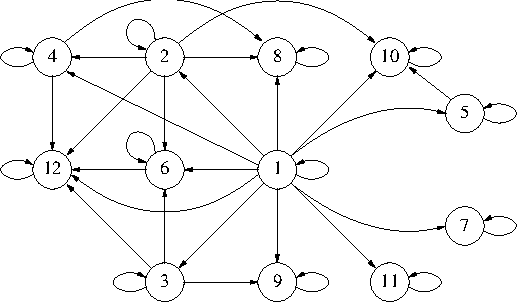
\includegraphics{figures/divisibility.pdf}
\caption{The Digraph for Divisibility on $\set{1,2,\dots,12}$.}
\label{fig:divisibility-digraph}
\end{figure}

%\hfill
%\includegraphics{divi2.pdf}
%{figures/divide12.mps}

%USE LATER: We use the notation $\diredge{a}{b}$ as an alternative notation for the
%pair $(a,b)$.

\section{Walks in Digraphs}\label{walks}

You take a walk through a digraph by starting at some point, following an
arrow from it to another point, and continue this way until you get tired.
For example in graph, $D$, of Figure~\ref{picdigraphg}, you might start at
$\mtt{x1}$, follow the arrow to $\mtt{x3}$, then follow the arrow back to
$\mtt{x1}$, and continue to $\mtt{x6}$ and then to $\mtt{x2}$ ---at which
point you're stuck because there's no arrow out of $\mtt{x2}$.

We can represent a walk by listing the starting point, followd by the successive
edges and points it goes through.  So your walk would be represented by the
sequence
\[
\mtt{x1, (x1,x3), x3, (x3,x1), x1, (x1,x6),x6,(x6,x2),x2}.
\]
This bloated representation may seem silly.  After all, either the sequence of
points, or the sequence of edges, determine what the walk is, so you don't
need both.  But this formal representation makes it correct to talk about
both the edges and the points on the walk,  which is convenient.  For
example, we can define the \term{length} of a walk to be the number of
occurrences of edges in it.  We can also say the walk \term{crosses itelf} when
there is a vertex that occurs more than once in the walk.
Walks that don't cross themselves are called \term{vertex-simple} walks.
A walk in which no edge appears more than once is called
\term{edge-simple}.

A walk is said to \term{connect} its starting vertex to its ending vertex,
we say vertex $u$ \term{is connected to} vertex $v$ when there is a walk
that connects $u$ to $v$.


and two 

If there is a walk 

\begin{definition}
A \emph{path in a relation}, $R$, is a sequence $a_0,\dots,a_k$ with $k \ge
0$ such that $a_i\, R\, a_{i+1}$ for every $0 \le i < k$.  The path is
said to \emph{start} at $a_0$, to \emph{end} at $a_k$ and the
\emph{length} of the path is defined to be $k$.
\end{definition}

Pictured as a digraph, a path $a_0,\dots,a_k$ in $R$ looks like a line
that starts at the point $a_0$ and follows arrows between successive
points on the path to end at $a_k$.  Note that a single point counts as a
length zero path (this is just for convenience).  A \emph{point-simple
path} is a path with no repeated points.  Likewise, an \emph{edge-simple
path} is a path in which no edge is used twice.  We usually just say
``simple path'' when we mean point-simple path (though Rosen uses ``simple
path'' to mean edge-simple.)



%inverse, composition, restriction

We can define some new relations based on paths.  Let $R$ be a relation on
a set, $A$.  For $n \in \naturals$ and $a,b \in A$, define relations
$R^{(n)}$, $R^{(\le n)}$, $R^+$, and $R^*$ on $A$ by the conditions that
\begin{eqnarray*}
a\, R^{(n)}\, b &\eqdef& \exists\mbox{ a path in $R$ from $a$ to $b$ of length $n$},\\
a\, R^{(\le n)}\, b &\eqdef& \exists\mbox{ a path in $R$ from $a$ to $b$ of
length $\le n$},\\
a\, R^+\, b &\eqdef& \exists\mbox{ a path in $R$ from $a$ to $b$ of length
$\ge 1$},\\
a\, R^*\, b &\eqdef& \exists\mbox{ a path in $R$ from $a$ to $b$}.\\
\end{eqnarray*}

Notice that $R^{(0)} = I_A$ because of the length-zero paths.  Also, $R =
R^{(1)}$ by definition of length-one path.

$R^*$ is called the \emph{path relation} of $R$.  It follows from the
definition of path that $R^*$ is transitive.  It is also reflexive (because
of the length-zero paths) and contains $R$ (because of the length-one
paths).  $R^+$ is called the \emph{positive-length path relation}; it also
contains $R$ and is transitive.


\iffalse

\subsection{Paths in Digraphs}\label{paths}

Pictured with points and arrows, a length $k$ path in a digraph looks like
a line that starts at a point, $a_0$, and traverses $k$ arrows between
successive points, $a_1,a_2,\dots$ to end at a point, $a_k$.  Note that
$k$ may be 0 ---a single vertex counts as length zero path to itself, just
as for simple graphs.  The precise definitions are very similar to those
for simple graphs:

\begin{definition}
A \emph{path in a digraph} is a sequence of vertices $a_0,\dots,a_k$ with
$k \ge 0$ such that $\diredge{a_i}{a_{i+1}}$ is an edge for every $i \geq
0$ such that $i < k$.  The path is said to \emph{start} at $a_0$, to
\emph{end} at $a_k$, and the \emph{length} of the path is defined to be
$k$.  The path is \emph{simple} iff all the $a_i$'s are different, that
is, $a_i = a_j$ only if $i=j$.
\end{definition}
\fi

\iffalse

%%USE in poset chapter

Many of the relational properties have geometric descriptions in terms of
digraphs.  For example:
\begin{description}

\item[Reflexivity:] All vertices have self-loops (a \emph{self-loop} at a
vertex is an arrow going from the vertex back to itself).

\item[Irreflexivity:] No vertices have self-loops.

\item[Asymmetry:] No self-loops and at most one (directed) edge between
any two vertices.

\item[Symmetry:] A binary relation $R$ is
\hyperdef{graphs}{symmetric}{\term{symmetric}} iff $aRb$ implies $bRa$ for
all $a,b$ in the domain of $R$.  So if there is an edge from $a$ to $b$,
there is also one in the reverse direction.  So edges may as well be
represented without arrows, indicating that they can be followed in either
direction.

\item[Transitivity:] Short-circuits---for any path through the graph,
there is an arrow from the first vertex to the last vertex on the path.
\end{description}
\fi
\iffalse

We can define some new relations based on paths.  Let $R$ be the edge
relation of a digraph.  Define relations $R^*$ and $R^+$ on the vertices
by the conditions that for all vertices $a,b$:
\begin{eqnarray*}
a\, R^*\, b &\eqdef& \mbox{there is a path in $R$ from $a$ to $b$},\\
a\, R^+\, b &\eqdef& \mbox{there is a positive length path in $R$ from $a$ to $b$}.
\end{eqnarray*}

$R^*$ is callaed the \emph{path relation}\footnote{In many texts, $R^*$ is
  called the \emph{transitive closure} of $R$.} of $R$ \iffalse.  It
follows from the definition of path that $R^*$ is transitive.  It is also
reflexive (because of the length-zero paths)\fi $R^+$ is called the
\emph{positive-length path relation}.  Both path relations and include $R$
(because of the length-one paths).


\subsection{Computer Representations \iffalse
of DIgraph\fi
}

\TBA{Adjacency matrix}, list of edges, list of neighbors, connection matrix.
$R^k$ and matrix power. 

%%%%%%%%%%%%%%%%%%%%%%%%%%%%%%%%%%%%%%
%%FAll 04 ln4 
%%%%%%%%%%%%%%%%%%%%%%%%%%%%%%%%

\section{Representation}

There are a several standard ways of representing relations.  The
different representations tend to highlight different properties of the
relation.  For computations involving relations, different representations
typically offer differing efficiencies.  For finite relations, we usually
use some method that explicitly enumerates the graph of the relation such
as lists of pairs, adjacency lists, matrices, and graphs.

\subsection{Lists of pairs}

A finite relation from set $A$ to set~$B$ can be represented by a list of
all the pairs in its graph.

\begin{example} \label{ex:0123-abc}
Let $N$ be the relation from the set of integers $\set{0, 1, 2, 3}$ to the
set of characters $\set{\texttt{a,b,c}}$ with graph
\[
\set{(0,\texttt{a}), (0, \texttt{c}), (1, \texttt{c}), (2, \texttt{b}),
(1,\texttt{a})}.
\]
Then $N$ would be represented by the list
\begin{quote}
\texttt{((0 a) (0 c) (1 c) (2 b) (1 a))}.
\end{quote}
\end{example}

\begin{example}
The divisibility relation on natural numbers $\set{1,\dots,12}$ is
represented by the list:
\[\begin{array}{l}
\texttt{((1 1) (1 2) (1 3) (1 4) (1 5) (1 6) (1 7) (1 8) (1 9)}\\
\texttt{ (1 10) (1 11) (1 12) (2 2) (2 4) (2 6) (2 8) (2 10) (2 12)}\\
\texttt{ (3 3) (3 6) (3 9) (3 12) (4 4) (4 8) (4 12) (5 5) (5 10)}\\
\texttt{ (6 6) (6 12) (7 7) (8 8) (9 9) (10 10) (11 11) (12 12))}xo
\end{array}\]
\end{example}
\fi

\iffalse
The relational properties we have defined all have straightforward
descriptions in terms of the list representation.  For example,
to test if a relation is reflexive, we can check its list representation
to be sure its list contains every pair of the form $(a\ a)$.  We can
describe symmetry and transitivity similarly:

\begin{description}

\item[Reflexivity:] The list contains all pairs $(a\ a)$ for $a \in A$.

\item[Symmetry:] If the list contains $(a\ b)$ then it also contains $(b\ a)$.

\item[Transitivity:] If the list contains $(a\ b)$ and $(b\ c)$ then it
contains $(a\ c)$.
\end{description}

\subsection{Adjacency Lists}

In an adjacency list representation, we list, for each element in the
domain, the elements in the codomain that it is related to.
\begin{example}
anLet $N$ be the relation from Example~\ref{ex:0123-abc}.
Then $N$ would be represented by the adjacency list
\begin{quote}
\texttt{((0 (a c)) (1 (c a)) (2 (b)) (3 ()))}
\end{quote}
\end{example}

Note that the adjacency list representation of a relation, $R$, is 
simply the list-of-pairs representation of the function on the domain of
$R$ that maps $a$ to the set $aR$.
\fi

\subsection{Connection Matrices}

Connection matrices are Boolean (0-1-valued) matrices that provide another
convenient computer representation for binary relations.  The
\emph{connection matrix} for a relation, $R$, from $A$ to $B$ has rows
labelled with the elements of $A$, columns labelled with elements of $B$,
and there is a 1 in row $a$, column $b$, iff $a\, R\, b$.  Otherwise the
$(a,b)$ entry is~0.
\begin{example}
The relation, $N$, from Example~\ref{ex:0123-abc} is represented by the
matrix
\[
\begin{array} {r|ccc}
& \texttt{a}& \texttt{b}&  \texttt{c} \\ 
\hline
0&1& 0&  1\\
1&1& 0&  1\\
2&0& 1&  0\\
3&0& 0&  0
\end{array}
\]
\end{example}

\begin{example}\label{divis12}
The divisibility relation over $\{1,2,\dots,12\}$ is 
represented by the matrix
\[
\begin{array}{r|cccccccccccc}
        &1  &2  &3  &4  &5  &6  &7  &8  &9 &10 &11 &12\\
      \hline
      1 &1  &1  &1  &1  &1  &1  &1  &1  &1  &1  &1  &1\\
      2 &0  &1  &0  &1  &0  &1  &0  &1  &0  &1  &0  &1\\
      3 &0  &0  &1  &0  &0  &1  &0  &0  &1  &0  &0  &1\\
      4 &0  &0  &0  &1  &0  &0  &0  &1  &0  &0  &0  &1\\
      5 &0  &0  &0  &0  &1  &0  &0  &0  &0  &1  &0  &0\\
      6 &0  &0  &0  &0  &0  &1  &0  &0  &0  &0  &0  &1\\
      7 &0  &0  &0  &0  &0  &0  &1  &0  &0  &0  &0  &0\\
      8 &0  &0  &0  &0  &0  &0  &0  &1  &0  &0  &0  &0\\
      9 &0  &0  &0  &0  &0  &0  &0  &0  &1  &0  &0  &0\\
      10&0  &0  &0  &0  &0  &0  &0  &0  &0  &1  &0  &0\\
      11&0  &0  &0  &0  &0  &0  &0  &0  &0  &0  &1  &0\\
      12&0  &0  &0  &0  &0  &0  &0  &0  &0  &0  &0  &1\\
    \end{array}
\]
\end{example}

\iffalse

Again, the relational properties we have defined can be described in terms
of the matrix representation for relations.  Namely, we look for the
following matrix properties:
\begin{description}

\item[Reflexivity:] 
The major (upper-left to lower-right) diagonal is all 1.
\item[Symmetry:] 
The matrix is unchanged by reflection about the major diagonal.
\item[Transitivity:] 
Not so obvious\dots
\end{description}
\fi

\subsection{Digraphs} 

A \emph{directed graph}, or \emph{digraph} for short, is exactly the same
as the graph of a binary relation, $R$, from $A$ to $B$, but we picture
the digraph geometrically by assuming there are different points on a
plane for the different elements of $A$ and $B$, with an arrow from the
point for $a$ to the point for $b$ exactly when $a\, R\, b$.

\begin{example}
Let $N$ be the relation from Example~\ref{ex:0123-abc}.  Then $N$ is
pictured by the following digraph:
\begin{center}\includegraphics{figures/0123abc.mps}\end{center}
\end{example}

Digraph pictures are mainly used for relations on a finite set $A$.

\begin{example}
\begin{samepage}
The divisibility relation over $\set{1,2,\dots,12}$ from
Example~\ref{divis12} is represented by the digraph
\begin{center}
\includegraphics{figures/divide12.mps}
\end{center}
\end{samepage}
\end{example}
\iffalse

Again, relational properties have natural explanations as geometric
properties.  For example:
\begin{description}

\item[Reflexivity:] 
All nodes have self-loops (a \emph{self-loop} at a point is an arrow
going from the point back to itself).

\item[Irreflexivity:] 
No nodes have self-loops.

\item[Symmetry:] 
All edges are bidirectional.

\item[Transitivity:] 
Short-circuits---for any path (sequence of consecutive arrows) through
the graph, there is a single arrow from the first to the last node.
\end{description}
nnn
\fi



\section{Operations on Relations}

\subsection{Set operations}
Since relations, more precisely their graphs, are sets, we automatically
inherit various operations on relations from set operations.  For example, 
the intersection, $R_1 \intersect R_2$ of relations $R_1, R_2$ is defined
to be the relation with
\begin{eqnarray*}
\graph{R_1 \intersect R_2} &\eqdef& \graph{R_1} \intersect \graph{R_2},\\
\domain{R_1 \intersect R_2} &\eqdef& \domain{R_1} \intersect
\domain{R_2},\\ \codomain{R_1 \intersect R_2} &\eqdef& \codomain{R_1}
\intersect \codomain{R_2}.
\end{eqnarray*}
A similar definition holds for $R_1 \union R_2$.

Intersections preserve several of the relational properties we have
considered.  It follows immediately from the definitions that if $R_1$ and
$R_2$ are both transitive, then so is $R_1 \intersect R_2$.  The same
holds for symmetry, reflexivity, and antisymmetry.  This implies that if
$R_1$ and $R_2$ are both partial orders, then so is $R_1 \intersect R_2$.
Likewise for being an equivalence relation.

Closely related to intersection is \hyperdef{def}{restrictrel}{the
restriction of a relation}.  If $R$ is a binary relation, on a set, $A$,
and $A_0 \subseteq A$ is a subset of $A$, then the \emph{restriction, $R
\restrict A_0$, of $R$ to $A_0$} is the binary relation with domain $A_0$
in which the elements of $A_0$ are related as they were under $R$.
Formally, the restriction is simply given by
\[
\graph{R \restrict A_0} \eqdef \graph{R} \intersect (A_0 \cross A_0).
\]

Restrictions also preserve transitivity, symmetry, reflexivity, and
antisymmetry, and so if $R$ is a partial order, so is any restriction of
$R$; likewise for being an equivalence relation.

\begin{problem}
Show that restrictions preserve the property of being a total order.  Show
that intersections do not always preserve totality.
\end{problem}

The union operation allows us to write an equation that describes the
obvious connection between the path relations $R^+$ and $R^*$ and the
length-$n$ path relations, $R^{(n)}$.  Namely,
\begin{eqnarray}
R^* &=& R^{(0)} \union  R^{(1)} \union R^{(2)} \union \cdots,\label{R*u}\\
R^+ &=&                 R^{(1)} \union R^{(2)} \union \cdots.\label{R+u}
\end{eqnarray}

The complement, $\bar{R}$, of a relation, $R$ is defined to be the
relation with the same domain and codomain as $R$ such that
\[
\graph{\bar{R}} \eqdef \domain{R}\cross\codomain{R} - \graph{R}.
\]

We similarly inherit relations on relations.  For example, the
\emph{containment relation} on relations is defined by the rule that $R_1$
is contained in $R_2$, in symbols, $R_1 \subseteq R_2$, iff the domain,
codomain and graph of $R_1$ are subsets, respectively, of the domain,
codomain and graph of $R_2$.  Sometimes the assertion ``$R_1$ implies
$R_2$'' is used to mean that $R_1$ is contained in $R_2$.  The reason is
that if $R_1 \subseteq R_2$, then
\[
a\, R_1\, b \text{  implies  } a\, R_2\, b.
\]

For example, we can now characterize $R^+$ as the \emph{smallest} (under
$\subseteq$) relation with the properties that
\begin{enumerate}
\item $R \subseteq R^+$,
\item $R^+$ is transitive.
\end{enumerate}
For this reason, $R^+$ is called the \emph{transitive closure} of $R$.
Similarly, the path relation, $R^*$, is called the \emph{reflexive,
transitive closure} of $R$.

\subsection{Products}
\hyperdef{def}{productrel}{The product}, $R_1 \cross R_2$, of relations
$R_1$ and $R_2$ is defined to be the relation with
\begin{eqnarray*}
\domain{R_1 \cross R_2} &\eqdef& \domain{R_1} \cross \domain{R_2},\\
\codomain{R_1 \cross R_2} &\eqdef& \codomain{R_1} \cross \codomain{R_2},\\
(a_1,a_2)\, (R_1 \cross R_2)\, (b_1,b_2) &\text{iff}& a_1\, R_1\, b_1
\land a_2\, R_2\, b_2.
\end{eqnarray*}

\begin{example}
Define a relation, $Y$, on age-height pairs of being younger \emph{and}
shorter.  This is the relation on the set of pairs $(y,h)$ where $y$ is a
natural number $\le 2400$ which we interpret as an age in months, and $h$
is a natural number $\le 120$ describing height in inches.  We define $Y$
by the rule
\[
(y_1,h_1) Y (y_2,h_2) \qiff y_1 \le y_2 \land h_1 \le h_2.
\]
That is, $Y$ is the product of the $\le$-relation on ages and the
$\le$-relation on heights.
\end{example}

Products preserve several of the relational properties we have considered.
Namely, it's not hard to verify that if $R_1$ and $R_2$ are both
transitive, then so is $R_1 \cross R_2$.  The same holds for symmetry,
reflexivity, and antisymmetry.  This implies that if $R_1$ and $R_2$ are
both partial orders, then so is $R_1 \cross R_2$.  Likewise for being an
equivalence relation.

On the other hand, the property of being a total order is not preserved.
For example, the age-height relation $Y$ is the product of two total
orders, but it is not total.  For example, the age 240 months, height 68
inches pair, (240,68) and the age 228 months, height 72 inches pair,
(228,72) are incomparable under $Y$.

\subsection{Inverse}

The inverse, $R^{-1}$, of a relation, $R$, from $A$ to $B$ is just $R$
``turned backwards.''  Namely, $R^{-1}$ the relation from $B$ to $A$ such that
\[
b\, R^{-1}\, a \qiff a\, R\, b.
\]

The inverse operation has simple explanations in terms of the various
representations for relations.  For example, the connection matrix for
$R^{-1}$ is simply the \emph{transpose} (reflection around the major
diagonal) of the connection matrix for~$R$.  Note that the inverse of a
relation is not the same thing as the inverse of the matrix
representation.

The digraph picture for $R^{-1}$ is simply the picture for~$R$ with every
arrow reversed in direction.

\iffalse
If a function $f:A\to B$ is a bijection (\cf Rosen), then
it has an unique inverse function, $f^{-1}: B \to A$ defined by the rule
that
\[
f(a) = b \qiff f^{-1}(b) = a.
\]
\fi


Inverse also preserves several of the relational properties we have
considered.  Namely, if $R$ is transitive, so is $R^{-1}$.  Likewise for
symmetry, reflexivity, and antisymmetry.  This implies that if $R$ is a
partial order, then so is $R^{-1}$.


\subsection{Composition}

Composition of relations generalizes composition of functions.  If
$R_1$ is a relation from $A$ to $B$ and $R_2$ is a relation from $B$ to
$C$, then the composition of $R_1$ and $R_2$ corresponds to using $R_1$ to
get from $A$ to $B$ and then $R_2$ to get from $B$ to $C$.

More precisely, the \emph{composition}, $R_2 \compose R_1$, of $R_1$ and
$R_2$---note the reversal in the order of $R_1$ and $R_2$
here\footnote{The symbol~$\compose$ is a constant source of confusion---if
you read a book you should always check how the authors define~$\compose$---
some of them define composition the other way around.}---is defined to be
the relation from $A$ to $C$ such that
\begin{displaymath}
a\, (R_2 \compose R_1)\, c  \qiff \exists b\, [a\, R_1\, b \land b\, R_2\, c].
\end{displaymath}

It's helpful to describe composition in terms of length-two paths in a
digraph.  Namely, $a\, (R_2 \compose R_1)\, c$ iff there is a length-two path
from $a$ to $c$ using an arrow from the point for $a$ in the digraph for
$R_1$, followed by an arrow to $c$ in the digraph for $R_2$.


\subsubsection{Relational Composition and Matrix Multiplication}

There is a lovely way to explain composition of relations using connection
matrices.  Namely, the connection matrix for the composition of two
relations $R_1$ and $R_2$ can be obtained by performing matrix
multiplication of the connection matrices of $R_2$ and $R_1$, except that
where the standard definition of matrix product calls for adding numbers,
we combine them with $\disj$ (Boolean OR).  This is called the \emph{Boolean
product} of the matrices.

That is, in ordinary matrix multiplication, the $(i,j)$th entry of the
matrix product is obtained by multiplying successive elements of the $i$th
row of the first matrix by the successive elements of $j$th column of the
second matrix, and adding up the resulting products of these pairs of
numbers.  If the original matrices are 0-1-valued, these products of
pairs will also be 0-1-valued, so it will make sense to $\lor$ them
together instead of adding them.

\begin{example}
Let $N$ be the relation from Example~\ref{ex:0123-abc}.  Its connection
matrix is
\[\begin{array}{r|ccc}
& \texttt{a}&  \texttt{b}&  \texttt{c}\\
\hline  
0& 1&  0&  1\\
1& 1&  0&  1\\
2& 0&  1&  0\\
3& 0&  0&  0
\end{array}
\]
Let $R$ be the relation from $\set{\texttt{a, b, c}}$ to
$\set{\texttt{d,e,f}}$ given by the connection matrix
\[\begin{array}{r|ccc}
& \texttt{d}&  \texttt{e}&  \texttt{f}\\
\hline  
\texttt{a}& 1&  1&  1\\
\texttt{b}& 0&  1&  0\\
\texttt{c}& 0&  0&  1
\end{array}
\]

The boolean product of these matrices is the matrix with rows labelled 0,
1, 2, 3 and columns labelled \texttt{d,e,f}.  To compute the
$(2,\texttt{e})$th entry in the product matrix, we take the 2-row of the
matrix for $N$:
\[
(0\ 1\  0)
\]
and the \texttt{e}-column of R:
\[
\left(\begin{array}{c}
1\\
1\\
0
\end{array}\right)
\]
and multiply corresponding entries to get the three products $0\cdot1, 1
\cdot 1$, and $0 \cdot 0$ and compute their disjunction:
\[
(0\cdot1) \disj (1 \cdot 1) \disj (0 \cdot 0) = 0 \disj 1 \disj 0 = 1.
\]
So the $(2,\texttt{e})$ entry is 1.  The complete product matrix is
\[\begin{array}{r|ccc}
& \texttt{d} &  \texttt{e} &  \texttt{f} \\
\hline  
0& 1&  1&  1\\
1& 1&  1&  1\\
2& 0&  1&  0\\
3& 0&  0&  0
\end{array}
\]
which is the connection matrix for $R \compose N$.
\end{example}

When $R$ is a relation on a set, $A$, it can be composed with itself.  The
composition $R \compose R$ of $R$ with itself is written $R^2$.  Similarly
$R^n$ denotes $R$ composed with itself $n$ times.  $R^n$ can be
recursively defined:
\begin{eqnarray*}
R^0 & \eqdef & I_A,\\
R^{n+1} & \eqdef & R \compose R^{n}.
\end{eqnarray*}

\begin{example}
\begin{samepage}
Consider the relation $R$ with graph $\set{(a,b), (a,c), (b,d), (d,e)}$.
The connection matrix and digraph for $R$ are:
    \begin{center}
      \begin{tabular}[b]{r|ccccc}
            &$a$&$b$&$c$&$d$&$e$ \\
        \hline
        $a$ & 0 & 1 & 1 & 0 & 0  \\
        $b$ & 0 & 0 & 0 & 1 & 0  \\
        $c$ & 0 & 0 & 0 & 0 & 0  \\
        $d$ & 0 & 0 & 0 & 0 & 1  \\
        $e$ & 0 & 0 & 0 & 0 & 0
      \end{tabular}
      \hfil
      \includegraphics{figures/tinyrel.mps}
    \end{center}    
  \end{samepage}
  \begin{samepage}
   For $R^2$ we have:
    \begin{center}
      \begin{tabular}[b]{r|ccccc}
            &$a$&$b$&$c$&$d$&$e$ \\
        \hline
        $a$ & 0 & 0 & 0 & 1 & 0  \\
        $b$ & 0 & 0 & 0 & 0 & 1  \\
        $c$ & 0 & 0 & 0 & 0 & 0  \\
        $d$ & 0 & 0 & 0 & 0 & 0  \\
        $e$ & 0 & 0 & 0 & 0 & 0
      \end{tabular}
      \hfil
      \includegraphics{figures/tinyrel2.mps}
    \end{center}
  \end{samepage}
  \begin{samepage}
   For $R^3$ we have:
    \begin{center}
      \begin{tabular}[b]{r|ccccc}
            &$a$&$b$&$c$&$d$&$e$ \\
        \hline
        $a$ & 0 & 0 & 0 & 0 & 1  \\
        $b$ & 0 & 0 & 0 & 0 & 0  \\
        $c$ & 0 & 0 & 0 & 0 & 0  \\
        $d$ & 0 & 0 & 0 & 0 & 0  \\
        $e$ & 0 & 0 & 0 & 0 & 0
      \end{tabular}
      \hfil
      \includegraphics{figures/tinyrel3.mps}
    \end{center}
  \end{samepage}
\end{example}

We claim that $R^n$ describes the length $n$ path relation of $R$.  That
is, $a\, R^n\, b$ iff there is a path in $R$ from $a$ to $b$ of
length $n$.  In other words:
\begin{lemma}\label{lem:Rn-paths}
\[
R^n = R^{(n)}
\]
\end{lemma}

\iffalse  %%PS or CP problem --not very interesting

\begin{proof}
By induction on $n$ with the statement of the Lemma as the induction
hypothesis, $P(n)$.

\textbf{Base case} $n=0$: We have that $a\, R^0\, b$ iff $a = b$ by
definition of $R^0$.  Also there is a length 0 path from $a$ to $b$ iff $a
= b$ by definition of length 0 path.  So $a\, R^0\, b$ iff there is a
length 0 path from $a$ to $b$.  That is, $R^0 = R^{(0)}$.

\textbf{Inductive step:} Suppose $P(n)$ holds for some $n\ge 0$.  We want
to prove $P(n+1)$.

First consider a length $n+1$ path $a=a_0,\dots,a_n,a_{n+1}=b$ in $R$.  By
induction hypothesis, we can assume that $a\, R^n\, a_n$.  Also, we have
by definition of path in $R$ that $a_n\, R\, b$.  Therefore,
\[
a\, (R \compose R^n)\, b
\]
by the definition of composition.  So $a\, R^{n+1} b$ by the recursive
definition of $R^{n+1}$.  This shows that $R^{(n+1)} \subseteq R^{n+1}$.

Conversely, suppose $a\, R^{n+1}\, b$.  By the definition of $R^{n+1}$,
there exists a $b'$ such that $a\, R^n\, b'$ and $b'\, R\, b$.  By the
inductive hypothesis, we can assume that there is a length $n$ path in $R$
from $a$ to $b'$.  But since $b'\, R\, b$, we can add $b$ to the end of
the path and obtain a length $n+1$ path from $a$ to $b$.  This shows that
$R^{n+1} \subseteq R^{(n+1)}$.

Hence, $R^{n+1} = R^{(n+1)}$, which is the statement $P(n+1)$, completing
the proof by induction.
\end{proof}
\fi

\subsubsection{Computing the Transitive Closure}

How do we actually find all the paths needed to compute the path relation
of a relation, say from its graph or connection matrix?  From
equation~(\ref{R*u}) and Lemma~\ref{lem:Rn-paths} we have
\[
R^* = R^0 \union  R^1 \union R^2 \union \cdots
\]

This helps since we know how to compute the composition $R^n$, but there
is still a problem: there are infinitely many terms!  When $A$ is finite,
however, we need only compute the first $\card{A}$ terms.

\begin{lemma}
Suppose $R$ is a relation on $A$.  Let $a$ and $b$ be elements of $A$ and
suppose that there is a path from $a$ to $b$ in $R$.  Then there is a path
of length at most $\card{A}-1$ from $a$ to $b$ in $R$.
\end{lemma}

\begin{proof}
We'll use the Least Number Principle.

Consider the shortest path $a=a_0,a_1,\dots,a_k=b$ from $a$ to $b$ (we
know one exists, so by the LNP there is a shortest one).  Suppose $k \ge
\card{A}$.  Then some element of $A$ appears twice in the list (with at
least $\card{A}+1$ list entries, one must be a repeat).  This means the
path is at some point circling back to where it was before.  We can cut
out this cycle from the path and get a shorter path.  This contradicts
that we had a shortest path.  So we cannot have $k \ge \card{A}$.
\end{proof}

\begin{corollary}
If $R$ is a relation on a set of size $n$, then
\[
R^* = \lgunion_{k=0}^{n-1} R^k.
\]
\end{corollary}

\begin{problem}
Prove that if $R$ is a relation on a finite set, $A$, then
\[
R^* = (R \union I_A)^{\card{A}}.
\]
\end{problem}

\iffalse

\subsection{Algebra of Relations}

With all these operations, there are no end of identities and other
connections among operations and properties of relations.  We don't really
need to develop these algebraic properties in this course, but we mention
without proof a small sample of algebraic facts about relational operators
just to offer a hint of the possibilities:
\begin{eqnarray*}
(R \union S)^{-1} & = & R^{-1} \union S^{-1},\\
(R \compose S)^{-1} & = & S^{-1} \compose R^{-1}\\
(R^*)^* & = & R^*\\
(R^{-1})^{-1} & = & R\\
(R^*)^{-1} & = & (R^{-1})^*\\
(R \intersect S) \cross T & = & (R \intersect T) \cross (S \intersect T)\\
(R \intersect S) \compose T & \subseteq & (R \compose T) \intersect (S \compose T)
\end{eqnarray*}
\fi

\iffalse

\section{Directed Acyclic Graphs}\label{sec:dag}

``Task graphs'' are a common source of partial orders: there is a set,
$A$, of tasks represented by points in the plane with an arrow from the
point for a task $a$ to the point for a task $b$ indicating that ``task
$a$ has to finish before task $b$ can begin.''

\begin{samepage}
\begin{example}\label{cloth}
Here is a graph that describes the order in which you could put on clothes.
The task are the clothes to be put on, and the edges say what should be put
on before what.
\begin{center}\includegraphics{figures/clothes.mps}\end{center}
\end{example}
\end{samepage}

This ``depends on'' graph imposes a partial ordering on tasks.  But what
if we add a relation edge from belt to underwear?  In that case the
dependency graph stops making sense: there is no way to get dressed!  What
goes wrong is that the added edge creates a ``cyclic'' dependency.

\begin{definition}
A \emph{cycle} is a positive length path in a digraph that begins and ends
at the same point.  A \emph{directed acyclic graph (DAG)} is a directed
graph with no cycles.
\end{definition}

So a task graph had better be a DAG for its tasks to be doable in an order
that respects task dependencies.

We use DAG's as an economical way to represent the dependency relation.
Usually a task-graph DAG itself is not a transitive relation because it
includes only the edges showing ``direct'' dependencies.  Rather, the
dependency relation we care about is defined by the positive length paths
in the task graph, that is, by transitive closure of the DAG.  The
\emph{dependency relation} of the DAG will always be a partial order:

\begin{lemma}
If $D$ is a DAG, then $D^+$ is a strict partial order.
\end{lemma}

\begin{proof}
We know that $D^+$ is transitive, so we just need to prove that it is
asymmetric.  We do so by contradiction.

Suppose that there exists $a,b$ such that $a\, D^+\, b$ and $b\, D^+\,
a$.  In other words, there is a path of positive length from $a$ to $b$
and also a path of positive length from $b$ to $a$ in $D$.  If we attach
these two paths, we get a path from $a$ to $a$ in $D$, that is, $D$
contains a cycle.  This contradicts the fact that $D$ has no cycles.
\end{proof}

\begin{problem}
Verify that any strict partial order is a DAG.

\solution{
Suppose the graph representation of a partial order $\prec$ has a cycle
$a_1,\dots,a_k,a_1$.  Then by transitivity of $\prec$ (with an induction
hiding inside) we have $a_1 \prec a_k$.  We also have $a_k \prec a_1$.
This violates the asymmetry of $\prec$, a contradiction.
}
\end{problem}


\begin{problem}
If $a$ and $b$ are distinct nodes of a digraph, then $a$ is said to
\emph{cover} $b$ if there is an edge from $a$ to $b$ and there is no other
path from $a$ to $b$.  If $a$ covers $b$, the edge from $a$ to $b$ is
called a covering edge.

\bparts

\ppart Show that if $D$ and $G$ are DAG's with the same transitive
closure, then they have the same set of covering edges.

\ppart Describe two graphs with nodes $\set{1,2,3}$ which have the same
transitive closure, but not the same set of covering edges.

\solution{In the graphs $\set{(1,2), (2,1), (2,3), (3,2)}$ and
$\set{(1,2).(2,3),(3,1)}$ all edges are covering edges.}

\ppart For any digraph, $D$, let $\widehat{D}$ be the subgraph of $D$
consisting of only the covering edges.  Show that if $D$ is finite and has
no self-loops, then $D$ and $\widehat{D}$ have the same transitive closure,
that is $D^+ = \widehat{D}^+$.
 
\ppart Conclude that if $D$ is a finite DAG, then $\widehat{D}$ has the
smallest number of edges among all digraphs with the same transitive
closure.

\ppart Show that the previous result is not true in general for infinite
DAG's. \hint An example of this kind has appeared several times in these
Notes.

\solution{In the DAG for $<$ on the reals, there are no covering edges, so
$\widehat{<}$ has no edges.}

\eparts
\end{problem}


\iffalse

\subsubsection{Hasse Diagrams}

If we draw the graph of a poset, we may get
\emph{lots} of edges (consider the $\le$ order on some natural
numbers).  But a lot of those edges are ``implicit'' from the
transitivity of the order. We can get a much less messy picture by
leaving out these arrows.

Consider the clothing example.  Under the transitive closure,
underwear precedes belt.  But we don't need to see that edge to know
it is there.
Similarly loops (which express reflexive relationships) aren't shown.
\begin{definition}
  A \emph{Hasse diagram} for a poset $(A,\preceq)$ is a graph: \\
 ---whose vertices are the elements of $A$, \\
 ---whose edges (arrows) represent pairs $(a,b)$, where $a \prec b$, \\
 ---if $ a \prec b$, the $a$ vertex is below the $b$ vertex, \\
 ---that contains no ``transitive edges'', \\
 ---for which all pairs in $\preceq$ are obtainable by transitivity from
  edges in the diagram.
\end{definition}
It's a ``transitive disclosure'' of the poset.
To convert the diagram above to an ``official form'' Hasse diagram,
we must remove the pants $\rightarrow$ jacket arrow:
\begin{center}\includegraphics{figures/clotheshasse.mps}\end{center}
\begin{samepage}
  The divisibility relation over $\{1,2,\dots,12\}$, represented by
  the digraph
  \begin{center}\includegraphics{figures/divide12.mps}\end{center}  
\end{samepage}
\begin{samepage}
  has the following Hasse diagram:
  \begin{center}\includegraphics{figures/divide12hasse.mps}\end{center}
\end{samepage}
\fi


% Examples:
% \begin{itemize}
% \item $S=\naturals, \preceq = \leq$,
% \item $S=\naturals, \preceq = \divides$, NOT because neither
%   $3\divides5$ nor $5\divides3$
% \item $S=P(\naturals), \preceq = \subseteq$, NOT because neither $\{3\}
%   \subseteq \{5\}$ nor $\{5\} \subseteq \{3\}$ 
% \item Lexicographic order on pairs of natural numbers, defined by:
%   $(a_1,a_2) \preceq (b_1,b_2)$ if and only if either $a_1 < b_1$,
%   or else $a_1 = b_1$ and $a_2 \leq b_2$. \\
%   $(2,37) \preceq (2,38) \preceq
%     (3,2)$.  ``Lexicographic'' because like dictionary.
% \end{itemize}

% This has been the basic material. \\
% Book has a bit more: \\
% lower bounds, upper bounds (for a subset---$\leq$ everything in the
% subset, or $\geq$) \\
% lub, glb, \\
% lattices. \\
% Read these parts. 

%%%%%%%%%%%%%%%%%%%%%%%%%%%%%%%%%%%%%%
%%END FAll 04 ln4 
%%%%%%%%%%%%%%%%%%%%%%%%%%%%%%%%
\fi

\subsection{Directed Acyclic Graphs}\label{sec:dag2}

\begin{definition}
A \emph{cycle} in a digraph is a path that begins and ends at the same
vertex.  Note that by convention, a single vertex is considered to be a
cycle of length 0 that begins and ends at the vertex.  A \emph{directed
acyclic graph (DAG)} is a directed graph with no positive length cycles.

A \emph{simple cycle} in a digraph is a cycle whose vertices are distinct
except for the beginning and end vertices.
\end{definition}

\iffalse
In contrast to undirected graphs, a single vertex \emph{is} considered to
be a simple cycle.
\fi
\iffalse

DAG's are an economical way to represent partial orders.  For example, the
\href{http://courses.csail.mit.edu/6.042/spring09/ln3.pdf#partial.orders}
{direct prerequisite} relation between MIT subjects described in Week 3
Notes was used to determine the partial order of indirect prerequisites on
subjects.  This indirect prerequisite partial order is precisely the
positive length path relation of the direct prerequisites.

\begin{lemma}
If $D$ is a DAG, then $D^+$ is a strict partial order.
\end{lemma}

\begin{proof}
We know that $D^+$ is transitive.  Also, a positive length path from a
vertex to itself would be a cycle, so there are no such paths.  This means
$D^+$ is irreflexive, which implies it is a strict partial order (see
\href{http://courses.csail.mit.edu/6.042/spring09/cp3r.pdf}{Week 3,
Wednesday, Class Problem 2}).
\end{proof}

It's easy to check that conversely, the graph of any strict partial order
is a DAG.

\begin{notesproblem}
Verify that any strict partial order is a DAG.

\solution{
Suppose the graph representation of a partial order $\prec$ has a cycle
$a_1,\dots,a_k,a_1$.  Then by transitivity of $\prec$ (with an induction
hiding inside) we have $a_1 \prec a_k$.  We also have $a_k \prec a_1$.
This violates the asymmetry of $\prec$, a contradiction.
}
\end{notesproblem}
\fi

The divisibility partial order can also be more economically represented by
the path relation in a DAG.  \hyperdef{divisibility}{DAG}{A DAG whose
\emph{path} relation is divisibility} on $\set{1,2,\dots,12}$ is shown in
Figure~\ref{fig:divisibility-DAG}; the arrowheads are omitted in the
Figure, and edges are understood to point upwards.

\begin{figure}[h]
%\centering \includegraphics{figures/divi2.pdf}
\begin{center}
\setlength{\unitlength}{1973sp}%
%
\begingroup\makeatletter\ifx\SetFigFont\undefined%
\gdef\SetFigFont#1#2#3#4#5{%
  \reset@font\fontsize{#1}{#2pt}%
  \fontfamily{#3}\fontseries{#4}\fontshape{#5}%
  \selectfont}%
\fi\endgroup%
\begin{picture}(5452,6034)(10475,-13269)
{\color[rgb]{0,0,0}\thinlines
\put(13210,-12952){\circle{618}}
}%
\put(13210,-13027){\makebox(0,0)[b]{\smash{{\SetFigFont{12}{24.0}{\rmdefault}{\mddefault}{\updefault}{\color[rgb]{0,0,0}1}%
}}}}
{\color[rgb]{0,0,0}\put(13192,-9352){\circle{618}}
}%
\put(13192,-9427){\makebox(0,0)[b]{\smash{{\SetFigFont{12}{24.0}{\rmdefault}{\mddefault}{\updefault}{\color[rgb]{0,0,0}4}%
}}}}
{\color[rgb]{0,0,0}\put(13192,-7552){\circle{618}}
}%
\put(13192,-7627){\makebox(0,0)[b]{\smash{{\SetFigFont{12}{24.0}{\rmdefault}{\mddefault}{\updefault}{\color[rgb]{0,0,0}8}%
}}}}
{\color[rgb]{0,0,0}\put(14410,-11170){\circle{618}}
}%
\put(14410,-11245){\makebox(0,0)[b]{\smash{{\SetFigFont{12}{24.0}{\rmdefault}{\mddefault}{\updefault}{\color[rgb]{0,0,0}5}%
}}}}
{\color[rgb]{0,0,0}\put(13810,-10252){\circle{618}}
}%
\put(13810,-10327){\makebox(0,0)[b]{\smash{{\SetFigFont{12}{24.0}{\rmdefault}{\mddefault}{\updefault}{\color[rgb]{0,0,0}10}%
}}}}
{\color[rgb]{0,0,0}\put(12592,-10252){\circle{618}}
}%
\put(12592,-10327){\makebox(0,0)[b]{\smash{{\SetFigFont{12}{24.0}{\rmdefault}{\mddefault}{\updefault}{\color[rgb]{0,0,0}6}%
}}}}
{\color[rgb]{0,0,0}\put(11992,-11170){\circle{618}}
}%
\put(11992,-11245){\makebox(0,0)[b]{\smash{{\SetFigFont{12}{24.0}{\rmdefault}{\mddefault}{\updefault}{\color[rgb]{0,0,0}3}%
}}}}
{\color[rgb]{0,0,0}\put(12592,-8452){\circle{618}}
}%
\put(12592,-8527){\makebox(0,0)[b]{\smash{{\SetFigFont{12}{24.0}{\rmdefault}{\mddefault}{\updefault}{\color[rgb]{0,0,0}12}%
}}}}
{\color[rgb]{0,0,0}\put(15610,-11152){\circle{618}}
}%
\put(15610,-11227){\makebox(0,0)[b]{\smash{{\SetFigFont{12}{24.0}{\rmdefault}{\mddefault}{\updefault}{\color[rgb]{0,0,0}7}%
}}}}
{\color[rgb]{0,0,0}\put(10792,-11170){\circle{618}}
}%
\put(10792,-11245){\makebox(0,0)[b]{\smash{{\SetFigFont{12}{24.0}{\rmdefault}{\mddefault}{\updefault}{\color[rgb]{0,0,0}11}%
}}}}
{\color[rgb]{0,0,0}\put(11992,-9370){\circle{618}}
}%
\put(11992,-9445){\makebox(0,0)[b]{\smash{{\SetFigFont{12}{24.0}{\rmdefault}{\mddefault}{\updefault}{\color[rgb]{0,0,0}9}%
}}}}
{\color[rgb]{0,0,0}\put(13210,-11152){\circle{618}}
}%
\put(13210,-11227){\makebox(0,0)[b]{\smash{{\SetFigFont{12}{24.0}{\rmdefault}{\mddefault}{\updefault}{\color[rgb]{0,0,0}2}%
}}}}
{\color[rgb]{0,0,0}\put(13201,-12661){\line( 0, 1){1200}}
}%
{\color[rgb]{0,0,0}\put(13201,-10861){\line( 0, 1){1200}}
}%
{\color[rgb]{0,0,0}\put(13201,-9061){\line( 0, 1){1200}}
}%
{\color[rgb]{0,0,0}\put(13201,-9061){\line( 0, 1){1200}}
}%
{\color[rgb]{0,0,0}\put(12601,-9961){\line( 0, 1){1200}}
}%
{\color[rgb]{0,0,0}\put(12001,-10861){\line( 0, 1){1200}}
}%
{\color[rgb]{0,0,0}\put(12901,-11161){\makebox(3.3333,23.3333){\SetFigFont{5}{6}{\rmdefault}{\mddefault}{\updefault}.}}
}%
{\color[rgb]{0,0,0}\multiput(14251,-10910)(-10.28143,13.70857){29}{\makebox(3.3333,23.3333){\SetFigFont{5}{6}{\rmdefault}{\mddefault}{\updefault}.}}
}%
{\color[rgb]{0,0,0}\multiput(13009,-10914)(-10.28143,13.70857){29}{\makebox(3.3333,23.3333){\SetFigFont{5}{6}{\rmdefault}{\mddefault}{\updefault}.}}
}%
{\color[rgb]{0,0,0}\multiput(13028,-9107)(-10.28143,13.70857){29}{\makebox(3.3333,23.3333){\SetFigFont{5}{6}{\rmdefault}{\mddefault}{\updefault}.}}
}%
{\color[rgb]{0,0,0}\multiput(12168,-10904)(10.28143,13.70857){29}{\makebox(3.3333,23.3333){\SetFigFont{5}{6}{\rmdefault}{\mddefault}{\updefault}.}}
}%
{\color[rgb]{0,0,0}\multiput(13387,-10884)(10.28143,13.70857){29}{\makebox(3.3333,23.3333){\SetFigFont{5}{6}{\rmdefault}{\mddefault}{\updefault}.}}
}%
{\color[rgb]{0,0,0}\put(13017,-12714){\line(-2, 3){861.692}}
}%
{\color[rgb]{0,0,0}\put(12915,-12863){\line(-4, 3){1943.360}}
}%
{\color[rgb]{0,0,0}\put(13425,-12739){\line( 2, 3){861.692}}
}%
{\color[rgb]{0,0,0}\put(13517,-12849){\line( 4, 3){1943.360}}
}%
\end{picture}%

\end{center}
\caption{A DAG whose Path Relation is Divisibility on $\set{1,2,\dots,12}$.}
\label{fig:divisibility-DAG}
\end{figure}

%%new for F09:

If we're using a DAG just as an economical way to picture or represent its
path relation, we might want to replace it with the minimum edge DAG with
the same path relation.  This minimum edge DAG order is unique and easy to
find (see problem~\ref{PS_min_edge_DAG}).

\begin{problems}
\homeworkproblems
\pinput{PS_min_edge_DAG}
\end{problems}


\endinput
